\subsection{Exact points: where the conductivity meets $\kappa$}
This graph places the two worked examples of the guide on the curves. The reach is not read off by eye: it is the suction where the conductivity curve of the soil crosses the horizontal line $K_r=\kappa$.
\begin{center}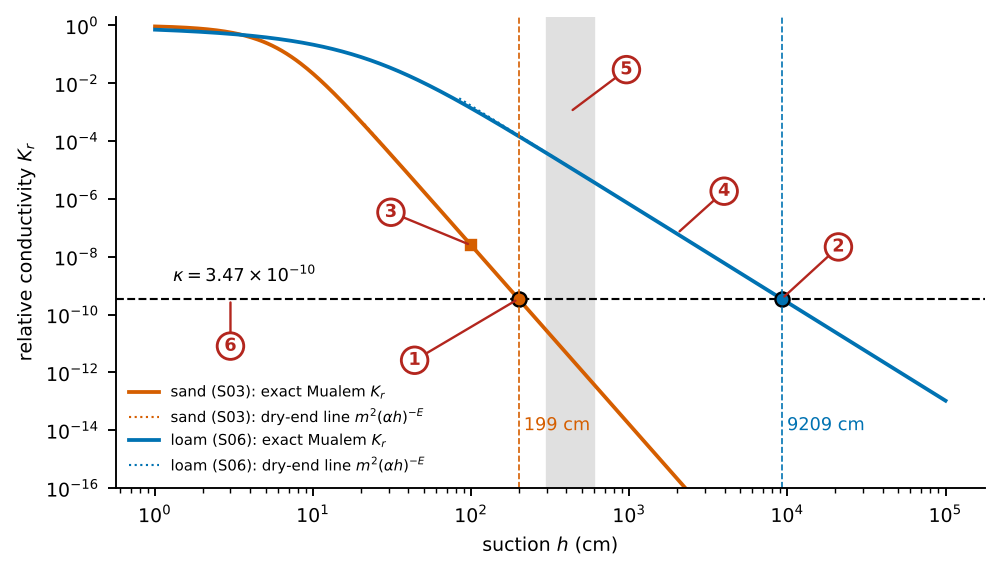
\includegraphics[width=0.92\textwidth]{../figures/paper4/ex_kr.png}\end{center}
\textbf{What the numbered labels point to, with the exact values.}
\begin{enumerate}[nosep,label=\protect\circled{\arabic*}]
\item Sand: the exact curve crosses the dashed line $K_r=\kappa$ at $h_c=199$\,cm (dot). This is \cref{eq:s-hc} with $\alpha=0.145$, $n=2.68$, $\ell=0.5$.
\item Loam: the crossing is at $h_c=9\,209$\,cm, just below $10^4$\,cm, with $\alpha=0.036$, $n=1.56$.
\item Sand at field capacity (100\,cm): $K_r=2.5\times10^{-8}$, a fraction of the saturated conductivity that is already tiny; the worked example of Part~2 of the guide.
\item Dotted lines: the dry-end straight line $m^2(\alpha h)^{-E}$. It lies on the exact curve wherever $\alpha h\gg1$, which is why the closed form of the reach is accurate.
\item Grey band (300--600\,cm): the usual triggers. They lie beyond the reach of sand and well inside the reach of loam.
\item The constant $\kappa$: the relative conductivity below which a crop can no longer dry the soil at the sensor within a season; one value for all ten soils.
\end{enumerate}
\textbf{How the exact points are obtained from the data.} The curves are the Mualem conductivity computed from $\alpha$ and $n$ of each soil (Table~A1 of the article, \nolinkurl{Manuscripts/results/p4_tableA1_reach.csv}). $\kappa$ is the fitted constant of \nolinkurl{p4_numbers.json} (key \texttt{kappa}), obtained from experiment E2 as shown in the next graph. The two crossings are computed with \cref{eq:s-hc}; the same numbers are in the workbook sheet \texttt{EQ\_P4\_reach}, cells of S03 and S06.
